\section{Zielsetzung}
Ziel des Versuches ist es, die Absorbtion von Gamma- und Beta-Strahlung bei verschiedenen Materialen zu untersuchen. 

\section{Theorie}
\label{sec:Theorie}

\subsection{Definition des Absorbtionskoeffizienten}
Der Wirkungsquerschnitt $\sigma$ stellt eine fiktive Fläche um ein stationäres Material dar, wobei eine Reaktion von dem einfallenden Teilchenstrahl mit einem stationären Teilchen genau dann eintrifft,
wenn es den Wirkungsquerschnitt trifft. Dies ist schematisch in Abbildung \ref{fig:WQ} gezeigt. Dabei ist $D$ die Dicke des Absorbers.


\begin{figure}[H]
    \centering
    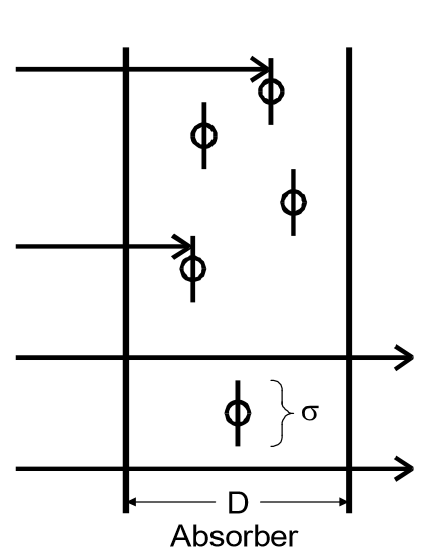
\includegraphics[width=5cm]{Bilder/WQ.png}
    \caption{Hier wird schematisch der Begriff des Wirkungsquerschnittes aufgezeigt.}
    \label{fig:WQ}
\end{figure}

\noindent Die Anzahl der Teilchen, die die Absorberschicht vollständig passieren, kann mit dem Absorbtionsgesetz

\begin{equation}
    N(D)=N_0 e^{-\mu D}
    \label{eqn:Absorberschicht}
\end{equation}
berechnet werden. 
Hier ist 
\begin{equation}
    \mu = n \sigma 
    \label{eqn:Absorbtionskoeffizient }
\end{equation}  \noindent als der Absorbtionskoeffizient definiert. 
Dabei ist $n$ die Anzahl der Teilchen in der Matrie und $N_0$ die Anzahl der eintreffenden Teilchen.


\subsection{Gamma-Strahlung}
Gamma-Strahlung besteht aus sehr energiereichen Photonen, entstanden durch en ergetische Übergänge von Atomkernen.
Diese sind in Ruhe masselos, besitzen aber einen Impuls und eine Energie.
Ihre Energie entsprich der des Übergangs im Atomkern, $\increment E$. 
Aufgrund ihrer Welleneigenschaften, kann man die Energie einese Photons auch über
\begin{equation*}
    E_\gamma=\frac{h c}{\lambda}
\end{equation*}
errechnet werden.
Beim Durchqueren des Absorbers kann ein $\gamma$-Quant auf mehrere verschiedene Arten mit der Matrie wechselwirken.
Hier werden nur die Relevantesten genannt.  

Bei dem Photoeffekt gibt ein Photon seine Energie an ein Hüllenelektron ab.
Dabei wird das Photon vernichtet und das Elektron aus der Atomhülle entfernt.
Der Wirkungsquerschnitt steigt hier mit $z^5$.
Das ist darauf zurückzuführen, dass die Bindungsenergie mit steigender Ordnungszahl $z$ ansteigt und der Photoeffekt abhängig von dieser ist.  


Bei dem Compton Effekt wird ein einfallendes Photon an einem freien Elektron gestreut.
Hier ändert sich die Energie und die Richtung des Photons.
Dies wird in der Abbildung \ref{fig:Compton} gezeigt.
Durch die Richtungsänderung ändert sich auch dei Intensität, da die selbe Menge an Photonen nach dem Absorber auf einen größeren Bereich verteilt sind.

\begin{figure}[H]
    \centering
    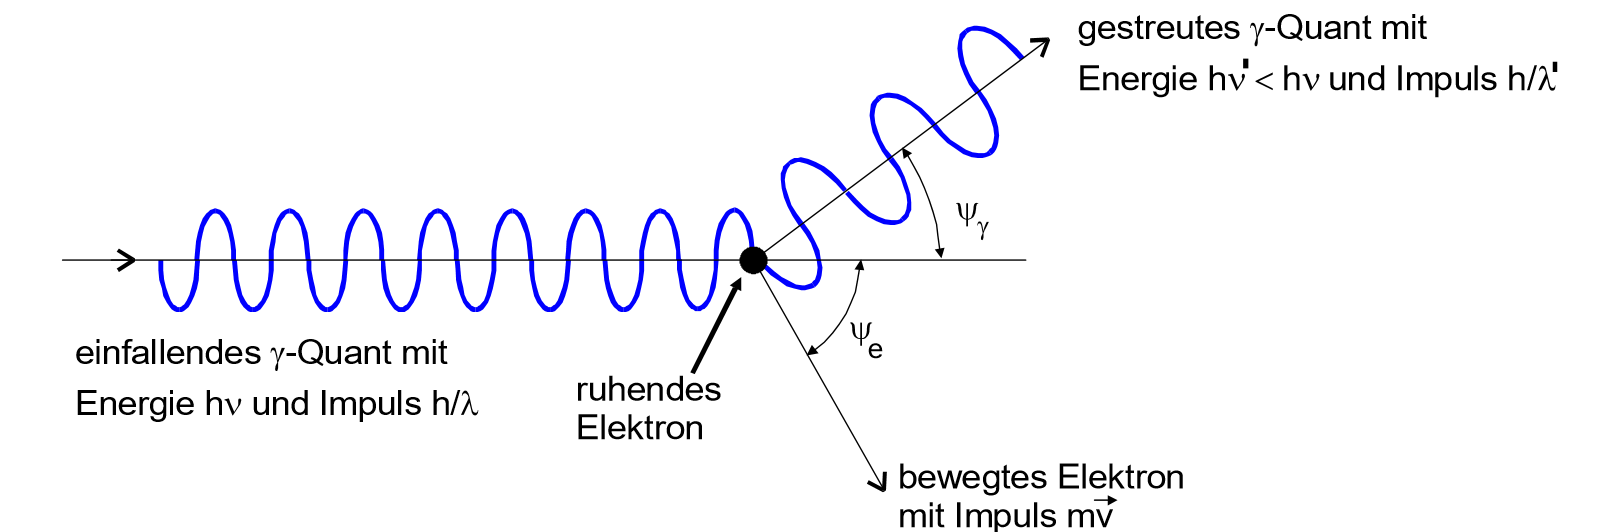
\includegraphics[width=\textwidth]{Bilder/Compton.png}
    \caption{Abgebildet ist ein Schema vom Compton Effekt.}
    \label{fig:Compton}
\end{figure}

\noindent Der Wirkungsquerschnitt kann mit
\begin{equation}
    \sigma_{com}=2 \pi r_e^2 \Bigl\{ \frac{1+\varepsilon}{\varepsilon^2}\Bigl[ \frac{2(1+\varepsilon)}{1+2 \varepsilon}-\frac{1}{\varepsilon} \ln(1+2 \varepsilon)\Bigr]
    +\frac{1}{2 \varepsilon} \ln(1+2 \varepsilon)-\frac{1+\varepsilon}{(1+2\varepsilon)^2}\Bigr\}
    \label{eqn:Compton}
\end{equation}
berechnet werden.
Dieser ist proportional zu $z$.  

Der dritte Prozess, der für den Absorbtionskoeffizienten relevant ist, ist die Paarerzeugung.
Dieser Prozess wird bei höheren Energien wichtiger.
Hier werden, wenn ein Photon eine Energie besitzt, die höher ist als die Ruheenergie von zwei Elektronen $E_e=\qty{1.02}{\mega\electronvolt}$, ein Elektron und ein Positron erzeugt.
Dieser Prozess ist außerdem proportional zu $z^2$.

Die Abhängigkeit des Absorbtionskoeffizienten von der Energie wird in Abbildung \ref{fig:Gamma} grafisch dargestellt.
\begin{figure}[H]
    \centering
    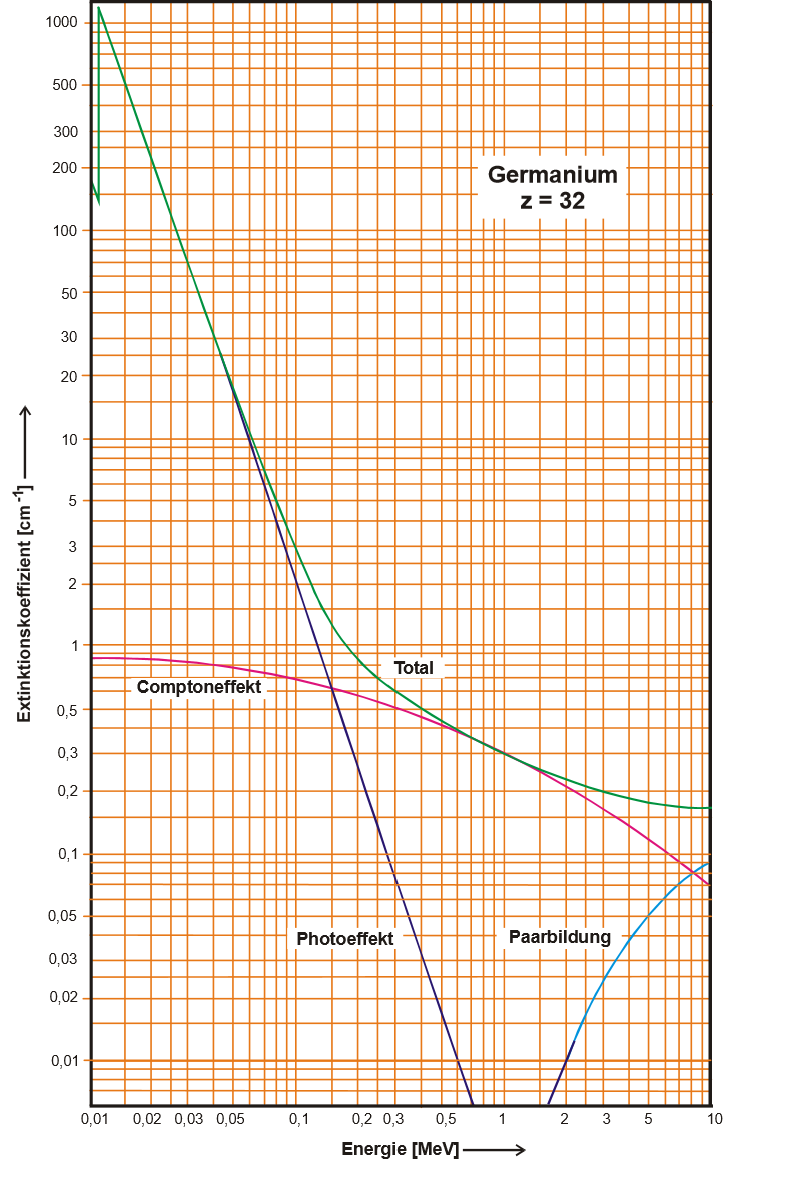
\includegraphics[width=8cm]{Bilder/Gamma.png}
    \caption{Abgebildet ist die der Absorbtionskoeffizient von Germanium abhängig von der Energie.}
    \label{fig:Gamma}
\end{figure}


\subsection{Beta-Strahlung}
Beta-Minus-Strahlung besteht aus hochenergetischen Elektronen, die durch die Umwandlung eines Neutrons in ein Proton entstehen.

\begin{equation*}
    \ce{n -> p + e- + \bar{\symup{\nu}}_e}
\end{equation*}
Die Energie, die bei der Umwandlung frei wurd, verteilt sich statistisch auf das Elektron und das Antineutrino $\bar{\symup{\nu}}_e$.
Dadurch entsteht das koninuierliche Spektrum in Abbildung \ref{fig:Beta}.

\begin{figure}[H]
    \centering
    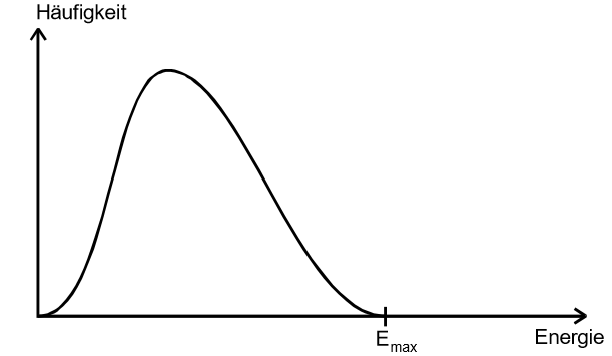
\includegraphics[width=10cm]{Bilder/Beta.png}
    \caption{Abgebildet ist das Emissionsspektrum von Beta-Strahlung.}
    \label{fig:Beta}
\end{figure}
Im Gegensatz zu Photonen besitzen Elektronen sowohl eine Ruhemasse, als auch eine Ladung.

Einer der Wechselwirkungsprozesse eines Elektrons mit der Matrie des Absorbers, ist die elastische Streuung an einem Atomkern, auch Rutherford-Streuung genannt.
Dabei werden die einfallenden Teilchen stark aufgefächert, was eine Intensitätsabnahme zur Folge hat.
Die Energieabnahme bei diesem Prozess ist nur gering.  

Durch die Coulomb-Wechselwirkung mit einem Atomkern wird ein Elektron beschleunigt.
Dadbei wird Bremsstrahlung frei.
Der Wirkungsquerschnitt lässt sich hier mit
\begin{equation}
    \sigma_{Br}=\alpha r_e^2 z^2
    \label{eqn:brems}
\end{equation}
beschreiben.
Für die Energie gilt
\begin{equation}
    E_{Br}=7\cdot10^{-4}z\cdot E_\beta^2
    \label{eqn:brems2}
\end{equation}
Diese Formel ist gültig bis zu einer Energie von $\qty{2500}{\kilo\electronvolt}$.
  
Inelastische Streuung der Elektron an den Elektronen der Absorberatome führt zu Ionisation und zur Anregung dieser.
Dabei gibt das einfallende Elektron einen kleinen Teil seiner Energie ab.
Ein Elektron führt, in einem hinreichend dicken Material, diesen Prozess so lange durch bis es den Absorber nicht mehr verlässt.
  
Eine durch diese Vorgänge resultierende Absorbtionskurve ist in \ref{fig:Beta2} aufgetragen.
Dabei ist 
\begin{equation}
    R=\rho D
    \label{eqn:Massenbelegung}
\end{equation}
die Massenbelegung.
Die Strahlenintensität ist abhängig von dieser aufgezeichnet.
Dabei stellt die gestrichelte Linie die Hintergrundstrahlung dar.
Als maximale Reichweite der Beta-Teilchen ist $R_{max}$ eingetragen.
\begin{figure}[H]
    \centering
    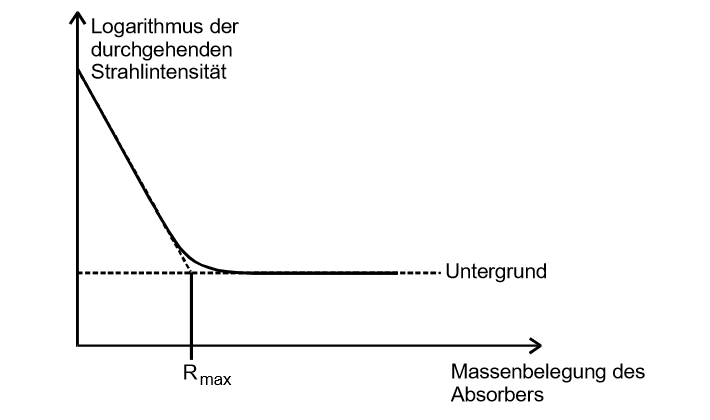
\includegraphics[width=10cm]{Bilder/Beta2.png}
    \caption{Aufgetragen ist die Absorbtionskurve von Beta-Strahlung.}
    \label{fig:Beta2}
\end{figure}
Mithilfe von $R_max$ und de Formel 
\begin{equation}
    E_{max}=1.92 \cdot \sqrt{R_{max}^2+0.22 \cdot R_{max}} [\unit{\mega\electronvolt}]
    \label{eqn:MaxEnergie}
\end{equation}
die maximale Energie der Beta-Teilchen berechnet werden.

\cite{V704}
